
\documentclass{standalone}
\usepackage[T1]{fontenc}
\usepackage[utf8]{inputenc}
\usepackage{pgf,tikz}

\begin{document}

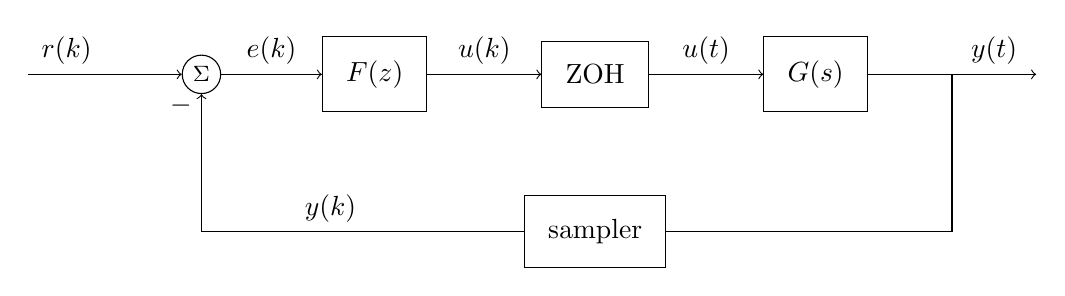
\begin{tikzpicture}[node distance=22mm, anchor=north]
  \node[coordinate] (input) {};
  \node[circle, draw, inner sep=2pt, right of=input] (sum) {\footnotesize $\Sigma$};
   \node[rectangle, draw, right of=sum, inner sep=3mm] (contr) {$F(z)$};
   \node[rectangle, draw, right of=contr, inner sep=3mm, node distance=28mm] (zoh) {ZOH};
   \node[rectangle, draw, right of=zoh, inner sep=3mm, node distance=28mm] (lti) {$G(s)$};
   \node[rectangle, draw, below of=zoh, inner sep=3mm, node distance=20mm] (sampler) {sampler};
   \node[coordinate, right of=lti, node distance=28mm] (output) {};
   \draw[->] (input) -- node[near start, above] {$r(k)$}  (sum);
   \draw[->] (sum) -- node[above] {$e(k)$}  (contr);
   \draw[->] (contr) -- node[above] {$u(k)$}  (zoh);
   \draw[->] (zoh) -- node[above] {$u(t)$}  (lti);
   \draw[->] (lti) -- node[coordinate] (meas) {} node[near end, above] {$y(t)$} (output);
   \draw[->] (meas) |- (sampler) -| node[above, pos=0.3] {$y(k)$} node[left, pos=0.96] {$-$} (sum);
 \end{tikzpicture}
\end{document}
